%!TEX root = ../ICR.tex
\chapter{Introducción \label{cap:Introduccion}}

\section{Planteamiento del problema}

En la era de la información digital, la interconexión global ha traído consigo un desafío sin precedentes: la propagación masiva de \gls{desinformacion}. Este fenómeno, que abarca desde \glspl{noticiafalsa} (\textit{fake news}) hasta diversas formas de \gls{fraudedigital}, representa una amenaza significativa para la estabilidad social, económica y democrática a nivel mundial.

Las \glspl{noticiafalsa}, definidas como información deliberadamente engañosa disfrazada de periodismo auténtico \cite{bondielli2019survey}, se difunden a través de redes sociales y medios digitales con el fin de manipular la opinión pública y el comportamiento de los individuos. La gravedad de esta problemática se ha intensificado exponencialmente con la sofisticación de los actores maliciosos, la democratización de herramientas de generación de contenido mediante \gls{ia} \cite{hu2024bad}, y la velocidad sin precedentes con la que la información se viraliza en el ecosistema digital.

\textbf{Es importante distinguir entre noticias falsas y fraude digital}: mientras que las \glspl{noticiafalsa} se enfocan en la manipulación de la información y la opinión pública a través de contenido periodístico falso, el \gls{fraudedigital} abarca un espectro más amplio de actividades maliciosas orientadas principalmente a obtener beneficios económicos o acceso no autorizado a información sensible. \textbf{Este proyecto se centra específicamente en la detección de noticias falsas}, aunque la metodología desarrollada podría ser replicada y adaptada para abordar otros tipos de fraude digital.

La investigación reciente ha documentado el impacto multidimensional de la desinformación, que va desde la distorsión de procesos democráticos \cite{ali2020posttruth} hasta la creación de pánico público durante crisis sanitarias como la pandemia de COVID-19 \cite{perez2020fake}. Paralelamente, el fraude digital ha evolucionado hacia formas cada vez más sofisticadas, aprovechando tanto vulnerabilidades técnicas como sesgos cognitivos humanos \cite{ali2021fake}.

\textbf{Desde la perspectiva de detección automatizada, la problemática se conceptualiza fundamentalmente como un problema de clasificación binaria}: determinar si un contenido dado es \textbf{confiable} (información verificada y legítima) o \textbf{no confiable} (contenido desinformativo). Esta simplificación, aunque reduce la complejidad natural del espectro de veracidad de la información, resulta práctica y efectiva para aplicaciones reales donde los usuarios requieren respuestas claras y accionables.

La desinformación contemporánea se manifiesta a través de múltiples modalidades con un impacto significativo en individuos, empresas y sociedades, como se ilustra en la Figura \ref{fig:mapa_problema}. Aunque el presente estudio se enfoca específicamente en noticias falsas, es relevante comprender el contexto más amplio del fraude digital para dimensionar la importancia de desarrollar metodologías transferibles:

\begin{itemize}
    \item \textbf{Noticias falsas generadas por \gls{ia}:} Contenido sintético creado por Grandes Modelos de Lenguaje (\glspl{gpt}) que imita el estilo periodístico legítimo \cite{su2023fake} - \textit{Foco principal de este proyecto}
    \item \textbf{Desinformación política dirigida:} Campañas coordinadas para influir en procesos electorales y opinión pública \cite{carcamo2021fake} - \textit{Aplicable con la metodología propuesta}
    \item \textbf{Fraude financiero digital:} Esquemas que explotan plataformas digitales y criptomonedas \cite{cao2020corporate} - \textit{Metodología transferible}
    \item \textbf{Fraude laboral en línea:} Ofertas de empleo falsas que buscan obtener información personal o financiera \cite{nasser2021online} - \textit{Metodología transferible}
    \item \textbf{Estafas de ingeniería social:} Técnicas sofisticadas que combinan información personal extraída de redes sociales con narrativas convincentes - \textit{Metodología transferible}
    \item \textbf{Desinformación en salud:} Información médica falsa que puede tener consecuencias directas en la salud pública \cite{pulido2020new} - \textit{Aplicable con la metodología propuesta}
    \item \textbf{\Glspl{deepfake}:} Contenido multimedia manipulado mediante técnicas de \gls{dl} - \textit{Requiere extensión multimodal}
    \item \textbf{\Glspl{bulo}:} Información falsa que se propaga viralmente en redes sociales - \textit{Aplicable con la metodología propuesta}
\end{itemize}

\begin{figure}[h!]
    \centering
    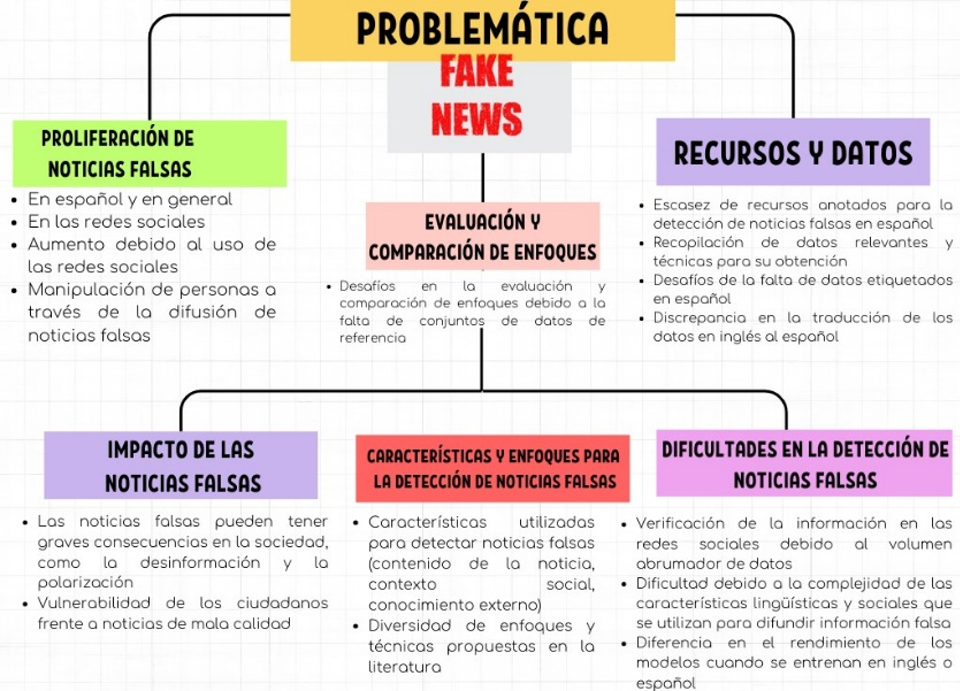
\includegraphics[width=\textwidth]{Imagenes/mapaConceptual1.png}
    \caption{Mapa Conceptual 1: Taxonomía del problema de desinformación con enfoque en noticias falsas y extensibilidad hacia fraude digital.}
    \label{fig:mapa_problema}
\end{figure}

\subsection{El Desafío Específico del Español}

El español, como la cuarta lengua más hablada del mundo con más de 500 millones de hablantes nativos \cite{acosta2019construccion}, presenta desafíos únicos para la detección automatizada de desinformación. A pesar de su importancia demográfica y económica, existe una notable escasez de recursos computacionales especializados para la detección de noticias falsas en español, en comparación con los abundantes recursos disponibles para el inglés \cite{posadas2019detection}.

Esta brecha de recursos se manifiesta en:
\begin{itemize}
    \item \textbf{Escasez de corpus etiquetados:} Limitados conjuntos de datos de entrenamiento en español para modelos de detección
    \item \textbf{Variabilidad dialectal:} La diversidad regional del español presenta desafíos adicionales para modelos generalizables
    \item \textbf{Contexto cultural específico:} Los patrones de desinformación varían según el contexto sociocultural hispanoamericano
    \item \textbf{Herramientas de detección limitadas:} Pocas soluciones tecnológicas disponibles para comunidades hispanohablantes
\end{itemize}

\subsection{La Complejidad Técnica del Problema}

La detección automatizada de \glspl{noticiafalsa} constituye un problema técnico multifacético que requiere la integración de múltiples disciplinas. Como documenta la literatura reciente \cite{singh2023comprehensive}, los desafíos incluyen:

\begin{itemize}
    \item \textbf{Análisis semántico profundo:} Necesidad de comprender el contexto y las implicaciones sutiles del contenido mediante técnicas de \gls{pln}
    \item \textbf{Detección de patrones estilométricos:} Identificación de características lingüísticas que indiquen autoría maliciosa \cite{tsai2023stylometric}
    \item \textbf{Procesamiento en tiempo real:} Capacidad de analizar el volumen masivo de contenido generado diariamente usando \gls{ml}
    \item \textbf{Adaptación a contenido sintético:} Detección de texto generado por modelos de \gls{ia} cada vez más sofisticados \cite{su2023adapting}
    \item \textbf{Robustez ante ataques adversariales:} Resistencia a intentos deliberados de evadir la detección
    \item \textbf{Optimización de \glspl{hiperparametro}:} Calibración de parámetros del modelo para maximizar el rendimiento
\end{itemize}

Dada la sofisticación de estas amenazas, se requieren soluciones tecnológicas igualmente avanzadas para combatir el fraude digital, como se esquematiza en la Figura \ref{fig:mapa_soluciones}. Este trabajo se centra en el desarrollo de tales soluciones, con un enfoque particular en el idioma español y la comparación sistemática de paradigmas tecnológicos complementarios.

\begin{figure}[h!]
    \centering
    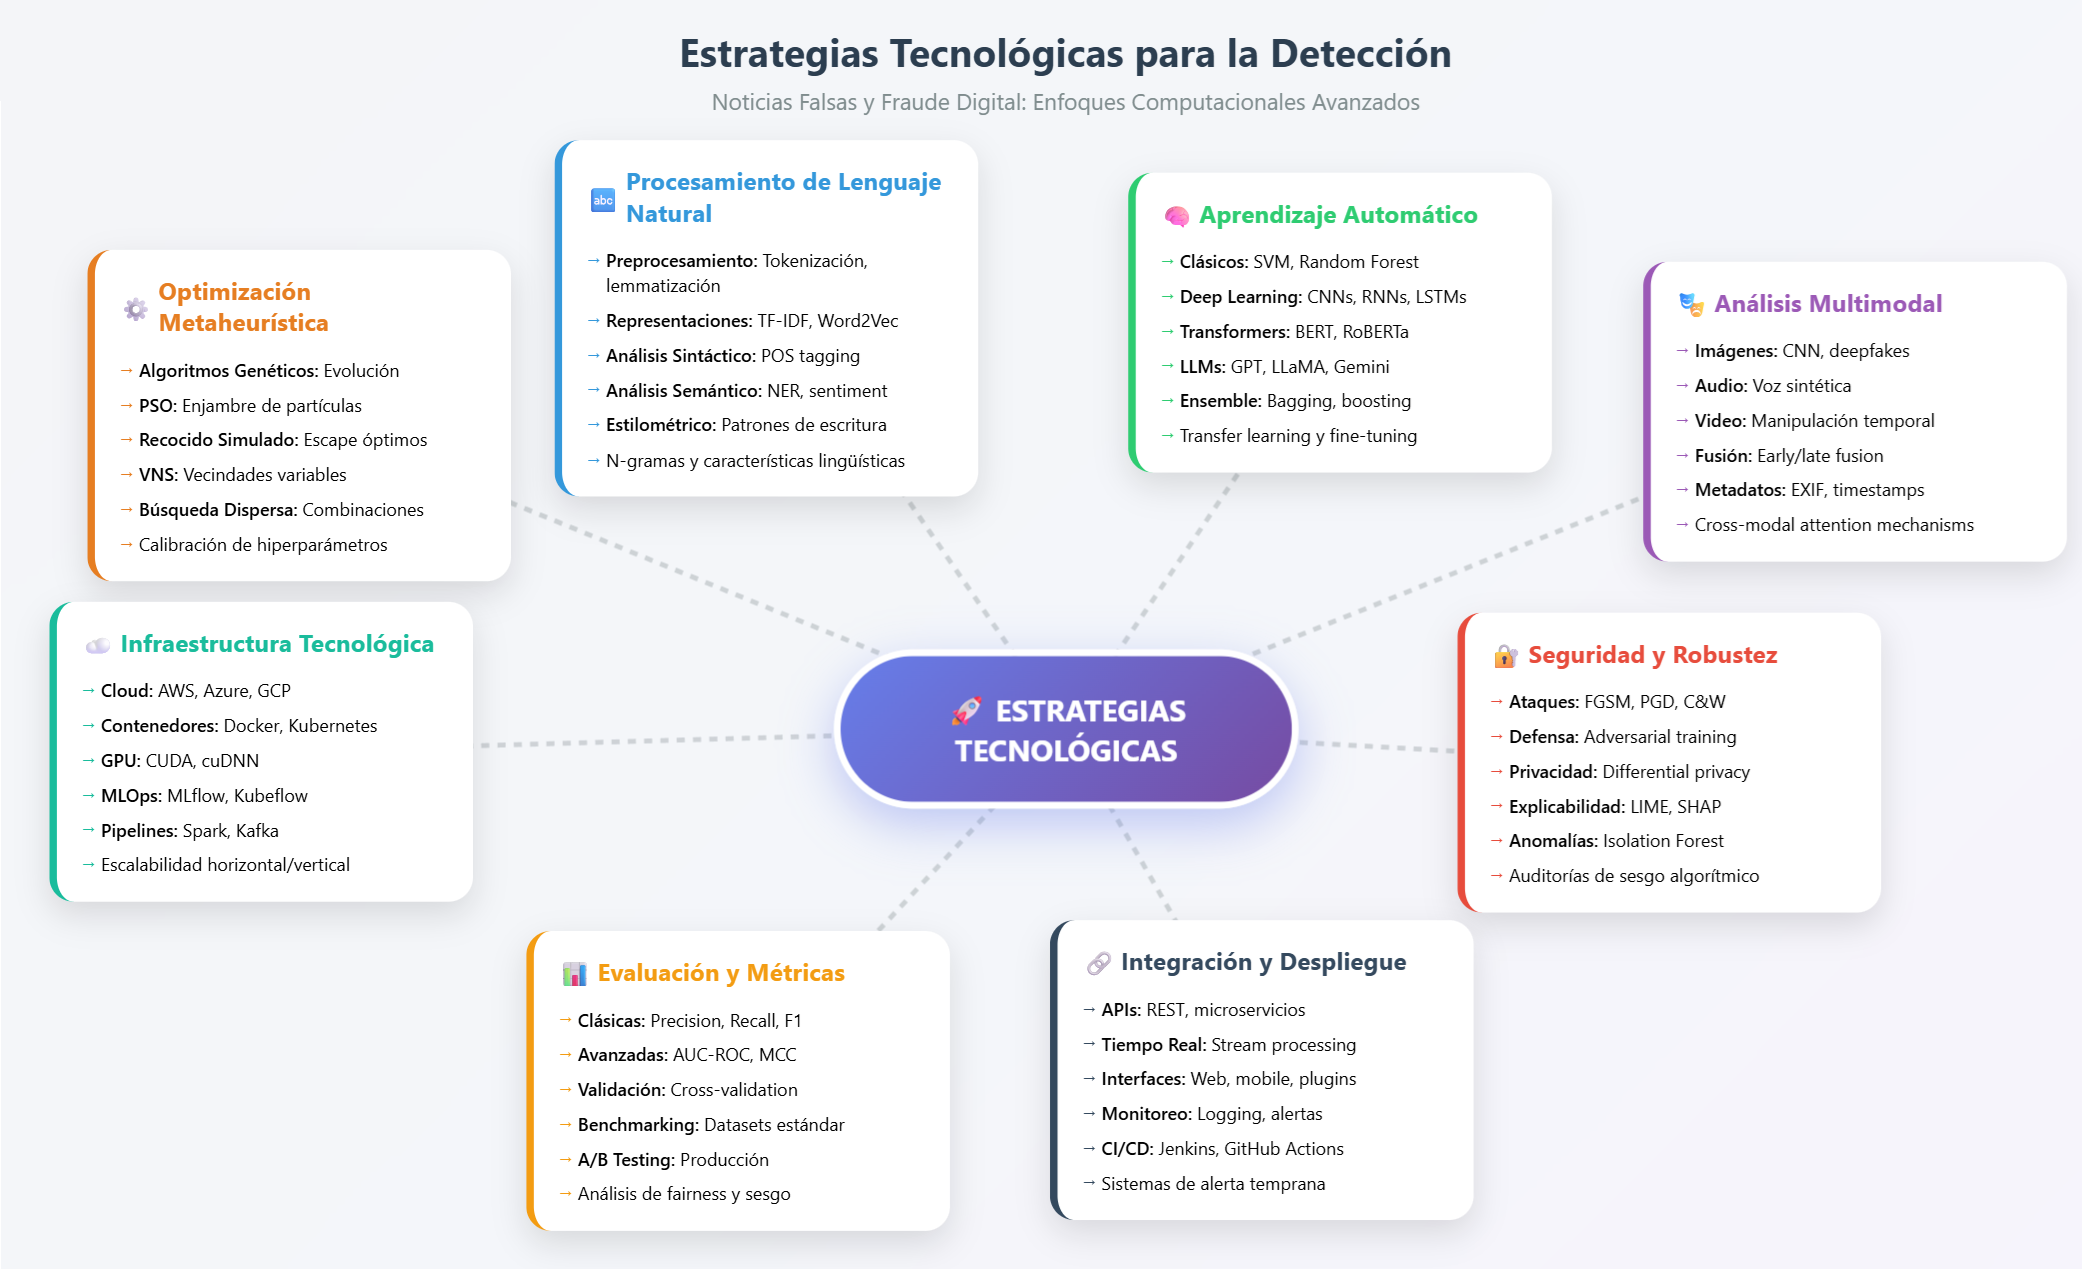
\includegraphics[width=\textwidth]{Imagenes/mapaConceptual2.png}
    \caption{Mapa Conceptual 2: Estrategias tecnológicas para la detección de fraude digital.}
    \label{fig:mapa_soluciones}
\end{figure}

\section{Motivación}

La motivación para llevar a cabo esta investigación se fundamenta en una combinación de experiencias personales observadas y la identificación de una brecha crítica en la protección tecnológica de las comunidades hispanohablantes.

\subsection{Impacto Personal y Social Observado}

Durante el desarrollo de esta investigación, se observaron múltiples casos en el entorno cercano donde personas fueron víctimas de fraude digital sofisticado. Estos casos incluyeron desde estafas de inversión disfrazadas de noticias financieras legítimas, hasta esquemas de phishing que aprovechaban eventos noticiosos actuales para parecer creíbles. Las víctimas, frecuentemente personas de edad avanzada o con menor exposición a tecnología digital, sufrieron no solo pérdidas económicas significativas, sino también impacto psicológico profundo, incluyendo sentimientos de vergüenza, ansiedad y pérdida de confianza en medios digitales.

\subsection{Vulnerabilidad de Poblaciones Específicas}

La investigación en psicología cognitiva aplicada a la desinformación \cite{ali2021fake} ha demostrado que ciertos grupos demográficos son particularmente vulnerables:

\begin{itemize}
    \item \textbf{Adultos mayores:} Mayor susceptibilidad a heurísticas de credibilidad basadas en autoridad percibida
    \item \textbf{Poblaciones con menor alfabetización digital:} Limitada capacidad para evaluar la legitimidad de fuentes online
    \item \textbf{Comunidades con acceso limitado a información:} Mayor dependencia de redes sociales como fuente primaria de noticias
    \item \textbf{Hablantes nativos de español:} Menor disponibilidad de herramientas de verificación en su idioma nativo
\end{itemize}

\subsection{Urgencia Tecnológica}

El rápido avance en modelos generativos de IA, como GPT-3 \cite{brown2020language} y sus sucesores, ha reducido significativamente las barreras técnicas para la creación de contenido falso convincente. Esta democratización de la capacidad de generar desinformación \cite{su2023fake} crea una urgencia imperativa para desarrollar defensas tecnológicas igualmente sofisticadas.

Impulsado por la necesidad de crear defensas tecnológicas más robustas y específicamente adaptadas para la comunidad hispanohablante, el presente trabajo se centra en desarrollar, comparar y validar métodos computacionales avanzados para la detección y prevención del fraude digital, con el objetivo final de contribuir a la protección de las poblaciones más vulnerables frente a estas amenazas emergentes.

\section{Justificación}

Esta investigación se justifica desde múltiples perspectivas: la brecha tecnológica existente, la novedad metodológica del enfoque, y la necesidad social de herramientas especializadas para el español.

\subsection{Brecha Tecnológica en Recursos para el Español}

El español, con más de 500 millones de hablantes nativos distribuidos en 21 países, representa un vasto ecosistema digital que ha sido históricamente subatendido en términos de herramientas especializadas para la detección de desinformación. Mientras que para el inglés existen múltiples conjuntos de datos de gran escala como LIAR, FakeNewsNet, y CREDBANK \cite{hu2022deep}, los recursos equivalentes en español son limitados y fragmentados.

El estado del arte actual en español se basa principalmente en cuatro corpus principales:
\begin{itemize}
    \item \textbf{Corpus de Acosta (2019):} 598 noticias \cite{acosta2019construccion}
    \item \textbf{Spanish Fake News Corpus:} 971 noticias \cite{posadas2019detection}
    \item \textbf{Corpus de Tretiakov (2022):} 1,958 noticias \cite{tretiakov2022detection}
    \item \textbf{Spanish Political Fake News:} 57,000+ noticias \cite{blanco2024enhancing}
\end{itemize}

Esta fragmentación crea una barrera significativa para el desarrollo de modelos robustos y generalizables.

\subsection{Novedad Metodológica: Enfoque Evolutivo Comparativo}

La novedad principal de esta investigación radica en su enfoque evolutivo que compara sistemáticamente dos paradigmas fundamentalmente diferentes de la Inteligencia Artificial en el mismo contexto aplicado:

\subsubsection{Paradigma Clásico Optimizado}
\begin{itemize}
    \item \textbf{Representación textual:} Bolsa de Palabras (BoW) con ponderación TF-IDF
    \item \textbf{Optimización:} Algoritmos metaheurísticos para calibración de hiperparámetros
    \item \textbf{Clasificador:} Máquina de Vectores de Soporte (SVM) optimizada
    \item \textbf{Ventajas:} Eficiencia computacional, interpretabilidad, menor dependencia de hardware especializado
\end{itemize}

\subsubsection{Paradigma de Deep Learning}
\begin{itemize}
    \item \textbf{Representación textual:} Embeddings contextuales dinámicos
    \item \textbf{Modelo base:} DistilBERT pre-entrenado \cite{sanh2019distilbert}
    \item \textbf{Técnica:} Fine-tuning con optimización de hiperparámetros
    \item \textbf{Ventajas:} Comprensión semántica profunda, captura de relaciones contextuales complejas
\end{itemize}

\subsection{Contribución Científica Multidimensional}

Esta investigación ofrece contribuciones en múltiples dimensiones:

\subsubsection{Contribución a Recursos Lingüísticos}
\begin{itemize}
    \item \textbf{Corpus unificado:} Integración y estandarización de los principales corpus en español
    \item \textbf{Metodología de unificación:} Protocolo replicable para integrar conjuntos de datos heterogéneos
    \item \textbf{Benchmarking:} Establecimiento de líneas base comparativas para futura investigación
\end{itemize}

\subsubsection{Contribución Metodológica}
\begin{itemize}
    \item \textbf{Optimización metaheurística:} Aplicación sistemática de algoritmos bio-inspirados para calibración de hiperparámetros en ambos paradigmas
    \item \textbf{Análisis comparativo riguroso:} Evaluación exhaustiva usando métricas múltiples y validación cruzada
    \item \textbf{Transferencia tecnológica:} Implementación práctica en aplicaciones web containerizadas
\end{itemize}

\subsubsection{Contribución Aplicada}
\begin{itemize}
    \item \textbf{Herramientas funcionales:} Aplicaciones web deployables para análisis en tiempo real
    \item \textbf{Código abierto:} Disponibilidad pública de implementaciones para reproducibilidad
    \item \textbf{Impacto social directo:} Herramientas utilizables por comunidades hispanohablantes
\end{itemize}

\subsection{Relevancia en el Contexto de LLMs}

Con el advenimiento de Grandes Modelos de Lenguaje como GPT-3 \cite{brown2020language}, LLaMA \cite{touvron2023llama}, y Gemini \cite{gemini2023family}, la generación de contenido sintético convincente se ha democratizado significativamente. Esta evolución hace que la investigación en detección sea más urgente y relevante, particularmente para idiomas como el español que han recibido menor atención en el desarrollo de contramedidas tecnológicas.

\section{Objetivos}

\subsection*{Objetivo General}
Desarrollar un método computacional basado en algoritmos metaheurísticos y modelos de lenguaje para detectar noticias falsas en español, con metodología transferible a otros tipos de fraude digital.

\subsection*{Objetivos Específicos}

\begin{itemize}
    \item Recopilar y procesar un conjunto de datos diverso a partir de múltiples corpus en español, y enriquecerlo mediante técnicas de \textit{extracción web} para entrenar y evaluar los sistemas de detección.
    
    \item Implementar un sistema de detección inicial que utilice técnicas de Procesamiento del Lenguaje Natural (Bolsa de Palabras) y algoritmos metaheurísticos.
    
    \item Desarrollar un sistema de detección avanzado mediante el ajuste fino (\textit{fine-tuning}) de un modelo de lenguaje profundo (\texttt{DistilBERT}), optimizando su rendimiento a través de la calibración de hiperparámetros.
    
    \item Realizar un análisis comparativo del rendimiento entre el enfoque metaheurístico y el modelo de lenguaje, utilizando un conjunto completo de métricas de evaluación (Exactitud, Precisión, Exhaustividad y F1-Score).
    
    \item Desarrollar un prototipo de aplicación web funcional, contenerizada con \texttt{Docker}, para demostrar la aplicabilidad práctica del modelo de mayor rendimiento en el análisis de URLs para categorizar contenido noticioso como falso o legítimo, con potencial de extensión hacia otros tipos de fraude digital.
\end{itemize}

\section{Alcance y Limitaciones}

\subsection{Alcance}

\subsubsection{Alcance Lingüístico y Cultural}
\begin{itemize}
    \item \textbf{Idioma objetivo:} El proyecto se centra exclusivamente en textos en español, abarcando múltiples variedades regionales representadas en los corpus utilizados
    \item \textbf{Dominio de aplicación:} Detección de noticias falsas como caso de uso principal, con extensibilidad demostrada hacia otros tipos de fraude digital
    \item \textbf{Contexto geográfico:} Cobertura de múltiples países hispanohablantes a través de los corpus integrados
\end{itemize}

\subsubsection{Alcance Técnico}
\begin{itemize}
    \item \textbf{Modalidad de datos:} Procesamiento exclusivo de contenido textual (no multimodal)
    \item \textbf{Tipo de clasificación:} Clasificación binaria supervisada (FALSO/REAL)
    \item \textbf{Dominio principal:} Detección de noticias falsas en español
    \item \textbf{Arquitecturas evaluadas:} Comparación sistemática entre enfoques clásicos optimizados y modelos Transformer
    \item \textbf{Implementación práctica:} Desarrollo de aplicaciones web funcionales y containerizadas
\end{itemize}

\subsubsection{Transferibilidad de la Metodología}
\begin{itemize}
    \item \textbf{Fraude financiero digital:} La metodología puede adaptarse para detectar esquemas de inversión fraudulentos, estafas de criptomonedas, y ofertas financieras falsas
    \item \textbf{Fraude laboral:} Aplicable para identificar ofertas de empleo falsas y esquemas de reclutamiento fraudulentos
    \item \textbf{Estafas de ingeniería social:} Útil para detectar contenido de phishing y esquemas de manipulación social
    \item \textbf{Desinformación temática específica:} Extensible a desinformación médica, científica, o política con ajustes de dominio
    \item \textbf{Limitaciones de transferencia:} Contenido multimodal (deepfakes de video/audio) requiere arquitecturas especializadas adicionales
\end{itemize}

\subsubsection{Alcance Metodológico}
\begin{itemize}
    \item \textbf{Optimización metaheurística:} Aplicación de tres algoritmos bio-inspirados para calibración de hiperparámetros
    \item \textbf{Validación experimental:} Uso de validación cruzada estratificada y métricas múltiples
    \item \textbf{Reproducibilidad:} Documentación completa y código fuente disponible
\end{itemize}

\subsection{Limitaciones}

\subsubsection{Limitaciones de Datos}
\begin{itemize}
    \item \textbf{Dependencia de corpus existentes:} El rendimiento está condicionado por la calidad y representatividad de los corpus disponibles en español
    \item \textbf{Sesgos inherentes:} Posibles sesgos temporales, temáticos o geográficos presentes en las fuentes originales
    \item \textbf{Evolución del lenguaje:} Los modelos pueden no capturar patrones emergentes en desinformación generada por IA más reciente
    \item \textbf{Etiquetado ground truth:} Dependencia de la calidad del etiquetado manual en los corpus originales
\end{itemize}

\subsubsection{Limitaciones Técnicas}
\begin{itemize}
    \item \textbf{Recursos computacionales:} El entrenamiento de modelos Transformer requiere hardware especializado (GPU) y tiempos de cómputo extensos (12-72+ horas)
    \item \textbf{Escalabilidad en tiempo real:} Los prototipos funcionan bajo demanda, no están optimizados para procesamiento de streams masivos
    \item \textbf{Generalización cross-domain:} Los modelos están específicamente entrenados para noticias, la efectividad en otros tipos de fraude digital es inferencial
    \item \textbf{Robustez adversarial:} No se evalúa específicamente la resistencia a ataques de evasión intencionales
\end{itemize}

\subsubsection{Limitaciones Operacionales}
\begin{itemize}
    \item \textbf{Herramienta de apoyo:} Los sistemas desarrollados son herramientas de apoyo a la decisión, no reemplazan el juicio humano experto
    \item \textbf{Verificación absoluta:} La determinación definitiva de veracidad puede requerir investigación periodística especializada
    \item \textbf{Contexto dinámico:} Los patrones de desinformación evolucionan constantemente, requiriendo actualización periódica de los modelos
    \item \textbf{Consideraciones éticas:} No se abordan explícitamente implicaciones de sesgo algorítmico o impacto en libertad de expresión
\end{itemize}

\subsubsection{Limitaciones de Evaluación}
\begin{itemize}
    \item \textbf{Métricas tradicionales:} La evaluación se basa en métricas estándar que pueden no capturar completamente la complejidad del problema
    \item \textbf{Validación temporal:} No se realiza validación temporal explícita con datos de períodos posteriores al entrenamiento
    \item \textbf{Análisis de errores:} El análisis cualitativo de errores es limitado debido al volumen de datos procesado
\end{itemize}

\section{Contribuciones Esperadas}

\subsection{Contribuciones Teóricas}
\begin{itemize}
    \item \textbf{Metodología comparativa:} Marco sistemático para comparar paradigmas clásicos y modernos en detección de desinformación
    \item \textbf{Optimización metaheurística:} Aplicación novedosa de algoritmos bio-inspirados para calibración de modelos Transformer
    \item \textbf{Análisis de trade-offs:} Caracterización cuantitativa de compromisos entre eficiencia computacional y rendimiento predictivo
\end{itemize}

\subsection{Contribuciones Prácticas}
\begin{itemize}
    \item \textbf{Corpus unificado:} Recurso consolidado para investigación futura en español
    \item \textbf{Herramientas funcionales:} Aplicaciones deployables para uso comunitario
    \item \textbf{Código abierto:} Implementaciones reproducibles y extensibles
\end{itemize}

\subsection{Contribuciones Sociales}
\begin{itemize}
    \item \textbf{Protección comunitaria:} Herramientas accesibles para comunidades hispanohablantes
    \item \textbf{Democratización tecnológica:} Reducción de la brecha digital en herramientas de verificación
    \item \textbf{Capacitación y concientización:} Contribución a la alfabetización digital en detección de desinformación
\end{itemize}

\section{Organización del Documento}

Este documento se estructura de manera lógica y progresiva para guiar al lector a través del proceso completo de investigación, desarrollo y evaluación:

\begin{itemize}
    \item \textbf{Capítulo 2 - Marco Teórico:} Establece los fundamentos teóricos que sustentan ambas metodologías, desde técnicas clásicas de representación textual hasta arquitecturas Transformer modernas, incluyendo principios de optimización metaheurística.

    \item \textbf{Capítulo 3 - Estado del Arte:} Presenta una revisión comprehensiva y organizada temáticamente de la literatura relevante, identificando brechas de conocimiento y posicionando esta investigación en el contexto científico actual.

    \item \textbf{Capítulo 4 - Metodología:} Detalla la metodología evolutiva seguida, desde la construcción del corpus unificado hasta la implementación y optimización de ambos paradigmas de detección.

    \item \textbf{Capítulo 5 - Análisis de Resultados:} Presenta y compara exhaustivamente los resultados obtenidos por ambas metodologías, incluyendo análisis estadístico, métricas de rendimiento y discusión de fortalezas y limitaciones.

    \item \textbf{Capítulo 6 - Implementación de Prototipo:} Describe la arquitectura, desarrollo y despliegue de las aplicaciones web funcionales que demuestran la viabilidad práctica de los modelos desarrollados.

    \item \textbf{Capítulo 7 - Conclusiones y Trabajo Futuro:} Sintetiza los hallazgos principales, evalúa el cumplimiento de objetivos, y propone direcciones específicas para investigación futura en el campo.
\end{itemize}

Cada capítulo se construye sobre los anteriores, manteniendo coherencia narrativa y técnica a lo largo del documento, mientras proporciona la profundidad analítica necesaria para validar las contribuciones científicas y prácticas de esta investigación.